\documentclass{IEEEcsmag}


\usepackage[colorlinks,urlcolor=blue,linkcolor=blue,citecolor=blue]{hyperref}

\usepackage{upmath}

\jvol{XX}
\jnum{XX}
\paper{8}
\jmonth{May/June}
\jname{IT Professional}
\pubyear{2021}

\newtheorem{theorem}{Theorem}
\newtheorem{lemma}{Lemma}


\setcounter{secnumdepth}{0}

\begin{document}

\sptitle{DEPARTMENT: HEAD}

\title{Title: No More Than Four Lines}

\author{First A. Author}
\affil{First Affiliation, City, (State), Postal Code, Country}

\author{Second Author, Jr.}
\affil{Second Affiliation, City, (State), Postal Code, Country}

\author{Third Author, III}
\affil{Third Affiliation, City, (State), Postal Code, Country}

\markboth{DEPARTMENT HEAD}{DEPARTMENT HEAD}

\begin{abstract}
\looseness-1Abstract text goes here. To find your publication's abstract word count limit, navigate to your magazine's homepage from \url{https://www.computer.org/csdl/magazines} and clickWrite for Us $>$Author Information. An abstract is a single paragraphthat summarizes the significant aspects of the manuscript. Often it indicates whether the manuscript is a report of new work, a review or overview, or a combination thereof. Do not cite references in the abstract. Papers must not have been published previouslyand must be targeted toward the general technical reader. Papers submitted for peer review (not departments or columns) must fit into the theme of an open Call for Papers or be submitted as a ``Regular'' paper. Some Computer Society (CS)magazines provide early access to full manuscript submissions by posting a preprint of the article at acceptance. Preprint articles are considered formally published and may be cited using their Digital Object Identifier (DOI). IEEE's Publishing Operations teamwill provide editorial and production services throughout the publication process.
\end{abstract}

\maketitle


\chapteri{T}he introduction should provide background information (including relevant references) and should indicate the purpose of the manuscript. Cite relevant work by others, including research outside your company. Place your work in perspective by referring to other research papers. Inclusion of statements at the end of the introduction regarding the organization of the manuscript can be helpful to the reader.


This document is a template for \LaTeX. If you are reading a paper or PDF version of this document, please download the electronic file, trans\_jour.tex, from the IEEE Web site at \url{http://www.ieee.org/authortools/trans_jour.tex} so you can use it to prepare your manuscript. If you would prefer to use LaTeX, download IEEE's LaTeX style and sample files from the same Web page. You can also explore using the Overleaf editor at {https://www.overleaf.com/blog/278-how-to-use-overleaf-with-ieee-collabratec-your-quick-guide-to-getting-started\#.xsVp6tpPkrKM9}. Please reffer the IEEEtran\_HOWTO.pdf is the complete guide of \LaTeX\ for manuscript preparation included with this stuff.


\section{COPYRIGHT AND CLEARANCE}

All CS Magazine authors must obtain clearance from IEEE Computer Society before submitting the final manuscript. The ``\href{https://apps.na.collabserv.com/wikis/home?lang=en-us#!/wiki/W18e544042a85_4b63_915a_1d1ed2cf8338/page/Publication\%20clearance}{Publication Clearance}'' wiki provides details about the procedure. Computer Society employees must use the \href{https://mc.manuscriptcentral.com/cs-ieee}{ScholarOne  Manuscripts Clearance} System to obtain publication approval.

\section{SECTIONS}

Sections following the introduction should present your results and findings. The body of the paper should be approximately 6,000 words. The manuscript should evolve so that each sentence, equation, figure, and table flow smoothly and logically from whatever precedes it. Relevant work by others, as well as relevant products from other companies, should be adequately and accurately cited. Sufficient support should be provided (or cited) for the assertions made and conclusions drawn.

Headings may be numbered or unnumbered (``1 Introduction'' and ``1.2 Numbered level 2 head''), with no ending punctuation. As demonstrated in this document, the initial paragraph after a headingis not indented.

\section{JOURNAL STYLE}

Use American English when writing your paper. The serial comma should be used (``a, b, and c'' not ``a, b and c''). In American English, periods and commas are within quotation marks, like ``this period.'' Other punctuation is ``outside''! The use of technical jargon, slang, and vague or informal English should be avoided. Generic technical terms should instead be used.

\subsection{Acronyms and Abbreviations}

All acronyms should be defined at first mention in the abstract and in the main text. Define in figures, tables, and footnotes only if not defined in the discussion of the figure/table. Acronyms consist of capital letters (except where salted with lowercase), but the terms they represent need not be given initial caps unless a proper name is involved (``central processing unit'' [CPU] but ``Fourier transform'' [FT]). Use of ``e.g.'' and ``i.e.'' okay, but refrain from using ``etc.'' It is preferable to use these abbreviations only in parentheses (e.g., like this).

\begin{quote}
ABBREVIATE UNITS OF TIME (s, min, hr, day, mo, yr) ONLY IN VIRGULE CONSTRUCTIONS (10~$\umu$g/hr) AND IN ARTWORK; OTHERWISE, SPELL OUT, E.G., 10 DAYS, 3 MONTHS, 25 MINUTES. UNITS OF MEASURE (Kb, MB, kWh, etc.) SHOULD ALWAYS BE ABBREVIATED WHEN USED WITH A NUMERAL. IF USED ALONE, SPELL OUT (``16 MB of RAM'' BUT ``THESE VALUES ARE MEASURED IN MICROMETERS'').
\end{quote}

\subsection{Numbers}

Spell out numerals that have no unit of measure or time (one, two, $\ldots$ ten), but always use numerals with units of time and measure. Some examples are as follows: 11 through 999; 1,000; 10,000; twentieth century; twofold, tenfold, 20-fold; 2 times; 0.2 cm; $p = .001$; 25\%; 10\% to 25\%.

\section{MATH AND EQUATIONS}

Scalar {\it variables} and {\it physical constants} should be italicized, and a bold (non-italics) font should be used for {\bf vectors} and {\bf matrices}. Do not italicize subscripts unless they are variables.

Equations should be either display (with a number in parentheses) or inline.   


Display equations should be flush left and numbered consecutively, with equation numbers in parentheses and flush right.

Be sure the symbols in your equation have been defined before the equation appears or immediately following. Please refer to ``Equation (1),'' not ``Eq. (1)'' or ``equation (1).''

Punctuate display equations when they are part of the sentence preceding it, as in
\begin{equation}
A=\pi r^2.
\end{equation}
In addition, if the text following the equation flows logically as a part of the display equation, 
\begin{equation}
A=\pi r^2,
\end{equation}
use ending punctuation (comma) after the display equation.

\section{LISTS}

Avoid using lists. Instead, use full sentences and flowing paragraphs. If you absolutely must use a list, use them rarely and keep them short:
\begin{itemize}
\item {\it Style for bulleted lists}---This is the style that should be used for bulleted lists.
	
\item {\it Punctuation in lists}---Each item in the list should end with a period, regardless of whether full sentences are used.
\end{itemize}

\section{GRAPHICAL ABSTRACTS}

This journal accepts graphical abstracts, and they must be peer reviewed, which means the graphical abstract must be submitted with the full paper. graphical abstracts and their specifications. Please read the additional information provided by \href{http://www.ieee.org/publications_standards/publications/graphical_abstract.pdf}{\underline{IEEE about graphical abstracts}}.


\begin{figure}
\centerline{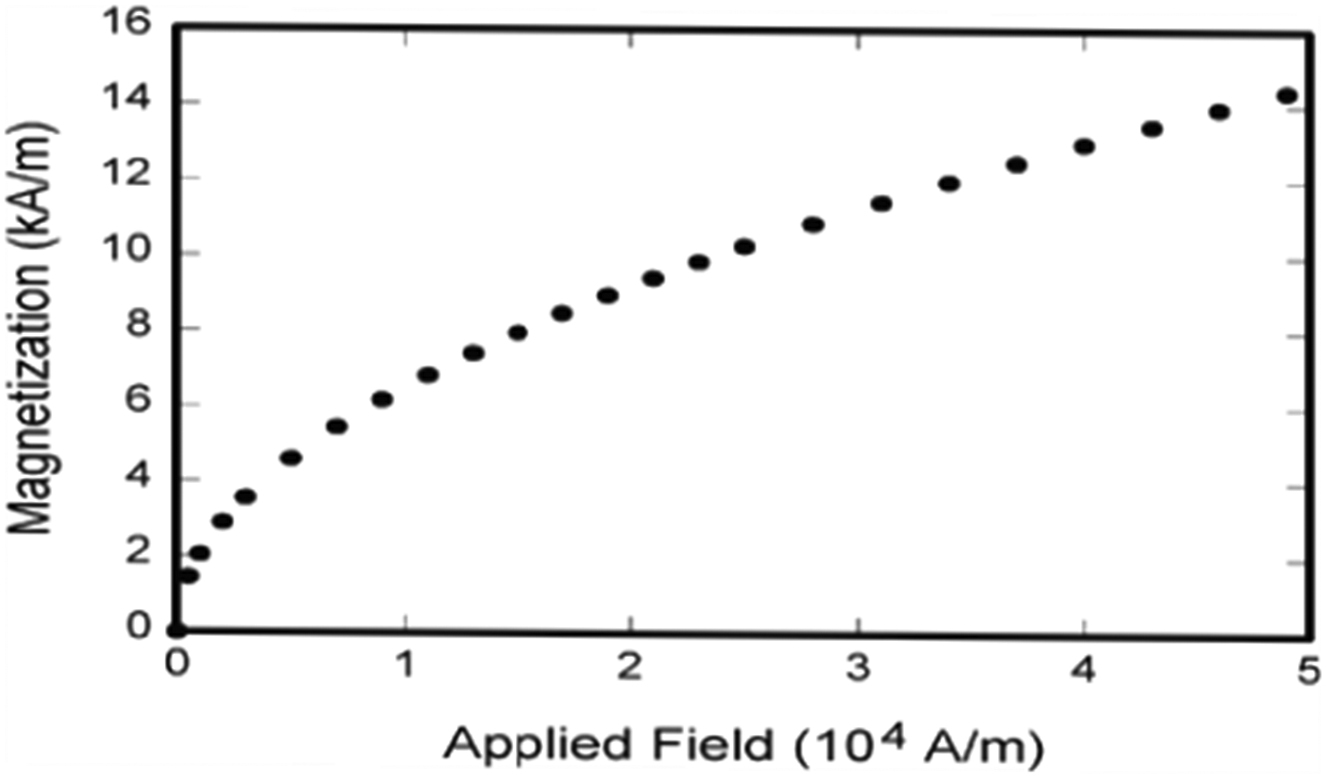
\includegraphics[width=18.5pc]{fig1.jpg}}
\caption{Note that ``Figure'' is spelled out. There is a period after the figure number, followed by one space. It is good practice to briefly explain the significance of the figure in the caption. (Used, with permission, from [4].)}
\end{figure}

\begin{figure*}
\centerline{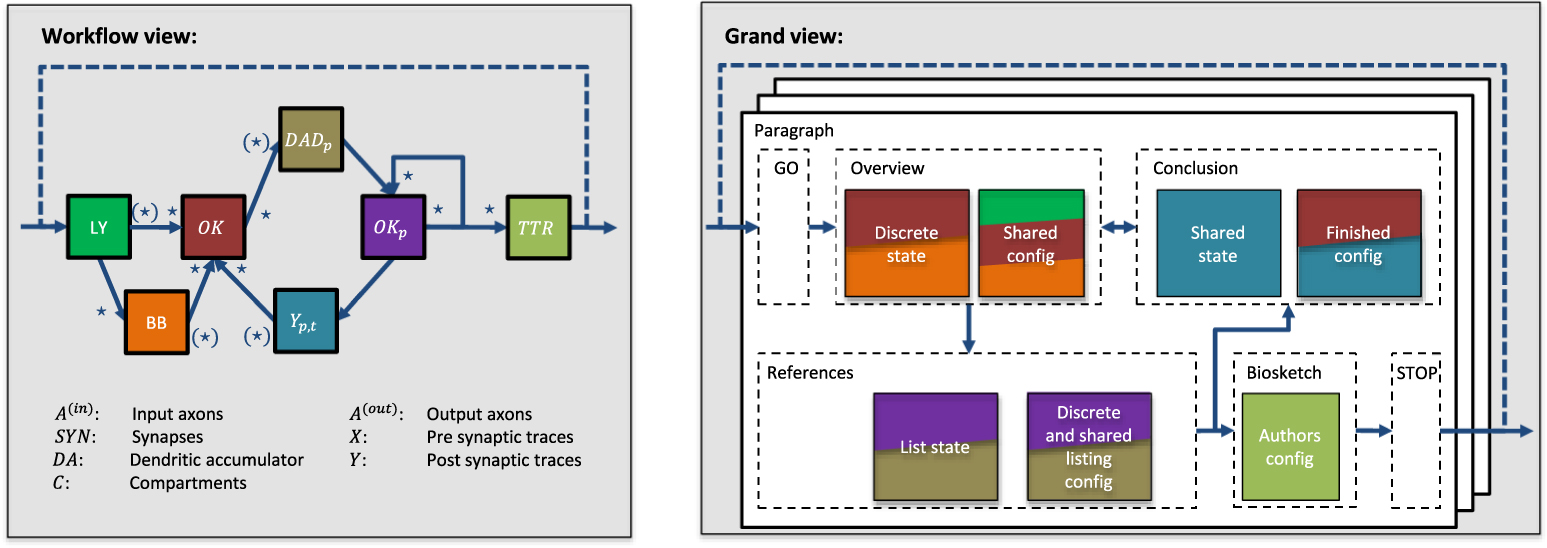
\includegraphics[width=26pc]{fig2.jpg}}
\caption{Note that ``Figure'' is spelled out. There is a period after the figure number, followed by one space. It is good practice to briefly explain the significance of the figure in the caption. (Used, with permission, from [4].)}
\end{figure*}

\begin{table}
\caption{Units for magnetic properties.}
\label{table}
\tablefont
\begin{tabular*}{17.5pc}{@{}p{29pt}p{63pt}<{\raggedright}p{80pt}<{\raggedright}@{}}
\toprule
Symbol& 
Quantity& 
Conversion from Gaussian and  CGS EMU to SI$^{\mathrm{a}}$ \\
\colrule
$\Phi $& 
Magnetic flux& 
1 Mx $\to  10^{-8}$ Wb $= 10^{-8}$ V $\cdot$ s \\
$B$& 
Magnetic flux density,   magnetic induction& 
1 G $\to  10^{-4}$ T $= 10^{-4}$ Wb/m$^{2}$ \\
$H$& 
Magnetic field strength& 
1 Oe $\to  10^{-3}/(4\pi )$ A/m \\
$m$& 
Magnetic moment& 
1 erg/G $=$ 1 emu   $\to 10^{-3}$ A $\cdot$ m$^{2} = 10^{-3}$ J/T \\
$M$& 
Magnetization& 
1 erg/(G $\cdot$ cm$^{3}) =$ 1 emu/cm$^{3}$   $\to 10^{-3}$ A/m \\
4$\pi M$& 
Magnetization& 
1 G $\to  10^{-3}/(4\pi )$ A/m \\
\botrule
\multicolumn{3}{@{}p{17.5pc}@{}}{$^{\mathrm{a}}$Gaussian units are the same as cg emu for magnetostatics; Mx 
$=$ maxwell, G $=$ gauss, Oe $=$ oersted; Wb $=$ weber, V $=$ volt, s $=$ 
second, T $=$ tesla, m $=$ meter, A $=$ ampere, J $=$ joule, kg $=$ 
kilogram, H $=$ henry.}
\end{tabular*}
\label{tab1}
\end{table}

\section{FIGURES AND TABLES}

\subsection{In-text Callouts for Figures and Tables}

Figures and tables must be cited in the running text in consecutive order. At first mention, the citation should be boldface ({\bf Figure 1}); subsequent mentions should be Roman type (see Figure 1 and {\bf Table 1}). {\bf Figure 2} shows an example of a figure spanning across two columns.
 

Previously published figures or tables require permission to reprint. Please obtain permission. Then, add the following text to the figure/table caption: ``From [reference no.], with permission,'' or ``Adapted from [reference no.], with permission.'' {\it Carefully} explain each figure in the text. Each manuscript should be limited to four figures.

\section{END SECTIONS}

\subsection{Appendices}

If multiple appendices are required, they should labeled ``Appendix A,'' ``Appendix B,'' etc. They appear before the ``Acknowledgment'' or the ``References'' section.

\subsection{Acknowledgment}

The ``Acknowledgment'' (no's) section appears immediately after the conclusion. If applicable, this is where you indicate funding for the work. The preferred spelling of the word ``acknowledgment'' in American English is without an ``e'' after the ``g.'' Avoid expressions such as ``One of us (S.B.A.) would like to thank $\ldots$ .'' Instead, write ``We thank $\ldots$.'' Sponsor and financial support acknowledgments are included in the acknowledgment section. For example: This work was supported in part by the U.S. Department of Commerce under Grant BS123456 (sponsor and financial support acknowledgment goes here). Researchers that contributed information or assistance to the article should also be acknowledged in this section. Also, if corresponding authorship is noted in your paper it will be placed in the acknowledgment section. Note that the acknowledgment section is placed at the end of the paper before the reference section.

\subsection{References}


References need not be cited in text. When they are, they appear on the 
line, in square brackets, inside the punctuation. Multiple references are 
each numbered with separate brackets. When citing a section in a book, 
please give the relevant page numbers. In text, refer simply to the 
reference number. Do not use ``Ref.'' or ``reference'' except at the 
beginning of a sentence: ``Reference \cite{CC1} shows $\ldots$ .'' Please do not use 
automatic endnotes in \emph{Word}, rather, type the reference list at the end of the 
paper using the ``References'' style.

Reference numbers are set flush left and form a column of their own, hanging 
out beyond the body of the reference. The reference numbers are on the line, 
end with period. In all references, the given name of the author 
or editor is abbreviated to the initial only and precedes the last name. Use 
them all; use \emph{et al.} only if names are not given. Use commas around Jr., 
Sr., and III in names. Abbreviate conference titles. When citing IEEE 
transactions, provide the issue number, page range, volume number, year, 
and/or month if available. When referencing a patent, provide the day and 
the month of issue, or application. References may not include all 
information; please obtain and include relevant information. Do not combine 
references. There must be only one reference with each number. If there is a 
URL included with the print reference, it can be included at the end of the\break 
reference. 

Other than books, capitalize only the first word in a paper title, except 
for proper nouns and element symbols. For papers published in translation 
journals, please give the English citation first, followed by the original 
foreign-language citation See the end of this document for formats and 
examples of common references. For a complete discussion of references and 
their formats, see the IEEE style manual at
\url{http://www.ieee.org/authortools}.

\section{CONCLUSION}

The manuscript should include a conclusion. In this section, summarize what was described in your paper. Future directions may also be included in this section. Authors are strongly encouraged not to reference multiple figures or tables in the conclusion; these should be referenced in the body of the paper.

\section{ACKNOWLEDGMENT}

We thank A, B, and C. This work was supported in part by a grant from XYZ.


\begin{thebibliography}{1}

\bibitem{AA1}
G. M. Amdahl, G. A. Blaauw, and F. P. Brooks, ``Architecture of the IBM System/360,'' {\it IBM J. Res. \& Dev}., vol. 8, no. 2, pp. 87--101, 1964. (journal)

\bibitem{BB1}
IBM Corporation, IBM Knowledge Center - IBM Secure Service Container (Secure Service Container). [Online]. Available: {https://www.ibm.com/support/\break knowledgecenter/en/HW11R/com.ibm.hwmca.kc\_se.doc/\break introductiontotheconsole/wn2131zaci.html} (URL)

\bibitem{CC1}
J. Williams, ``Narrow-band analyzer,'' PhD dissertation, Dept. of Electrical Eng., Harvard Univ., Cambridge, MA: 1993. (Thesis or dissertation)

\bibitem{DD1}
J. M. P. Martinez, R. B. Llavori, M. J. A. Cabo, et al., ``Integrating data warehouses with web data: A survey,'' {\it IEEE Trans. Knowledge and Data Eng}., preprint, Dec. 21, 2007, doi:10.1109/TKDE.2007.190746. (PrePrint)

\bibitem{EE1}
W.-K. Chen, {\it Linear Networks and Systems}, Belmont, CA: Wadsworth, pp. 123--135, 1993. (book)

\bibitem{FF1}
S. P. Bingulac, ``On the compatibility of adaptive controllers,'' {\it Proc. Fourth Ann. Allerton Conf. Circuits and Systems Theory}, pp. 8--16, 1994. (conference proceedings)

\bibitem{GG1}
K. Elissa, ``An overview of decision theory,'' unpublished. (Unpublished manuscript)

\bibitem{HH1}
R. Nicole, ``The last word on decision theory,'' {\it J. Computer Vision}, submitted for publication. (Pending publication)

\bibitem{II1}
C. J. Smith and J. S. Smith, Rocky Mountain Research Laboratories, Boulder, CO, personal communication, 1992. (Personal communication)
\end{thebibliography}


\begin{IEEEbiography}{First A. Author}{\,}current employment (is currently with XYZ Corporation, New York, NY). Author's latest degree received or which he/she is currently pursuing (He received the B.S. degree and the M.S. degree...."). Author's research interest. Association with any official journals or conferences; major professional and/or academic achievements, i.e., best paper awards, research grants, etc.; any publication information (number of papers and titles of books published). Author membership information, e.g., is a member of the IEEE and the IEEE Computer Society, if applicable, is noted at the end of the biography. Biography is limited to single paragraph only (He is a member of IEEE, etc.). All biographies should be limited to one paragraph, five to six sentences, consisting of the following: (e.g., ``Dr. Author received a B.S. degree and an M.S. degree $\ldots$ .''), including years achieved; association with any official journals or conferences; major professional and/or academic achievements, i.e., best paper awards, research grants, etc.; any publication information (number of papers and titles of books published); current research interests; association with any professional associations. Author membership information, e.g., is a member of the IEEE and the IEEE Computer Society, if applicable, is noted at the end of the biography. Contact him/her at faauthor@xyz.com.\vfill\pagebreak
\end{IEEEbiography}

\begin{IEEEbiography}{Second B. Author, Jr.,}{\,} with ABC Corporation, Böblingen, Germany. Ms. Author’s biography appears here.  Contact him/her at sbauthor@abc.com.
\end{IEEEbiography}

\begin{IEEEbiography}{Third C. Author, III,} {\,} with DEF Corporation, Tokyo, Japan. Dr. Author’s biography appears here.  Contact him/her at tcauthor@def.com.
\end{IEEEbiography}

\end{document}

